% Introduction


The gain in polularity of artifical intelligence in the recent years motivated our decision to build a smart lamp -- with machine learning as driving actor. The lamp ought to be smart enough to toggle itself \textbf{on} and \textbf{off}, solely based on data. Data which is collected at the beginning, in the so-called \emph{training-phase}, by manual user interaction with a physical switch.

Our concise two minute video (\url{https://www.youtube.com/watch?v=AOq6Cx7RbSw}) will give a short visual overview of the project.


\subsection{Hardware}

To keep monetary costs as low as possible, we tried using only the available hardware of prior excercises, i. e. a Raspberry Pi, several ESP32 developement boards and a broad range of available sensors+actors. But to avoid having to deal with mains electricity, because we as computer scientists should not act on exposed 230V wires with superficial knowledge, we were given three \emph{Phlips Hue}\footnote{\url{http://www2.meethue.com/de-DE}} lamps with a network bridge for control.

\subsection{Theoretical Layout}

The Raspberry Pi ended up as the projects control center. All sensory data, as well as onboard metrics like \emph{time of day} and \emph{daylight} are flowing to the Pi, where it is logged during the training-phase. The training-phase is exactly one week after first start-up or after initating a reset. After training-phase, the Raspberry Pi would query the trained model continuously with current sensor values, to decide wether to turn the lamp on or off.

Because the Pi is very limited in regards to RAM and processing power, we couldn't use a machine learning technique like deep neural networks to train the model. Whereas only classification would be possible. But because the model also had to be learned on the Pi itself, we moved away from the idea of a neural network and towards a decision tree.

Unlike a neural network, a decision tree requires discrete values, which forced us to lessen resolution of continuous values like \emph{time of day}. 

Following is the complete list of used metrics and their resolutions:

\begin{itemize}
    \item Time of Day
         \begin{itemize}
           \item Early Morning
           \item Morning
           \item Early Afternoon
           \item Late Afternoon
           \item Night
        \end{itemize}      
    \item Daylight
        \begin{itemize}
           \item True / False
        \end{itemize}    
    \item Weekday
     \begin{itemize}
           \item Mo -- So
        \end{itemize}   
    \item One entry per networked device
       \begin{itemize}
           \item Device Status (Connected, Disconnected)
          \end{itemize}
    \item Lamp Status
         \begin{itemize}
           \item On / Off
        \end{itemize}   
\end{itemize}

\begin{figure}
  \centering
    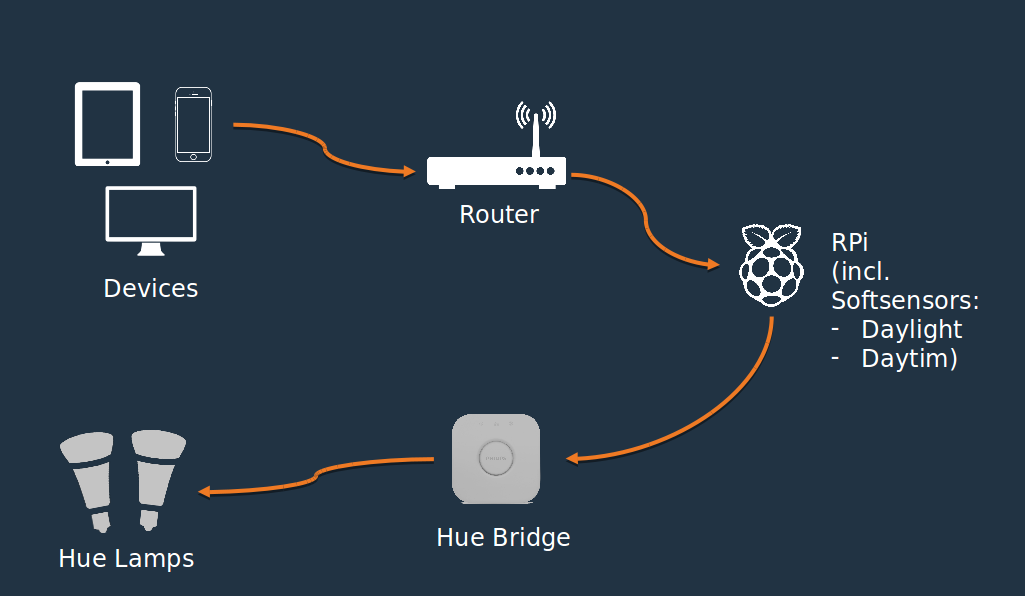
\includegraphics[width=1.0\textwidth]{../../ArchitectureFinal.png}
  \caption{Architecture}
  \label{fig:architecture}
\end{figure}
